%-----------------------------------------------------------------------------80
% CONTENT
%-----------------------------------------------------------------------------80
\subsection{Entorno de desarrollo Windows}


\begin{frame}[fragile]{Instalación de editor de código}
  \textbf{VS Code en Windows}
  \begin{itemize}[<+(1)->]
    \item Descargar el instalador desde \url{https://code.visualstudio.com/download}
  \end{itemize}  
    \begin{figure}
      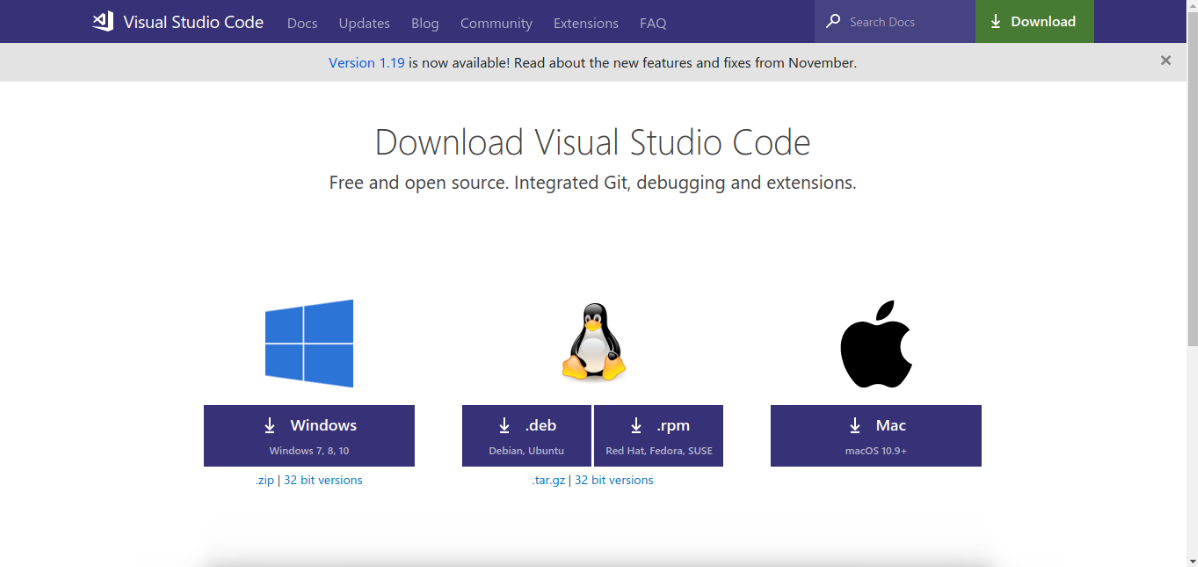
\includegraphics[width=1\textwidth]{./resources/1.png}
    \end{figure}

\end{frame}


\begin{frame}[fragile]{Instalación de editor de código}
  \textbf{VS Code en Windows}
  \begin{itemize}[<+(1)->]
    \item Iniciado el instalador, click en siguiente.
  \end{itemize} 
    \begin{figure}
      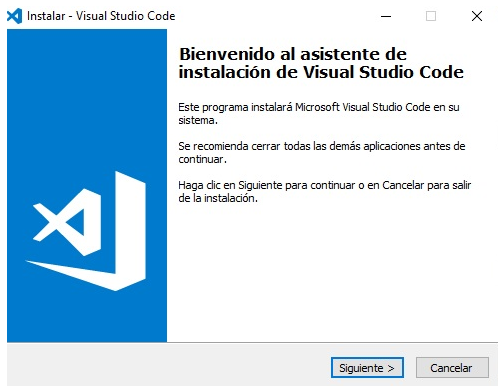
\includegraphics[width=1\textwidth]{./resources/2.png}
    \end{figure}
\end{frame}

\begin{frame}[fragile]{Instalación de editor de código}
  \textbf{VS Code en Windows}
  \begin{itemize}[<+(1)->]
    \item En la siguiente ventana, marcar de preferencia las opciones mostradas.
  \end{itemize} 
  \begin{figure}
    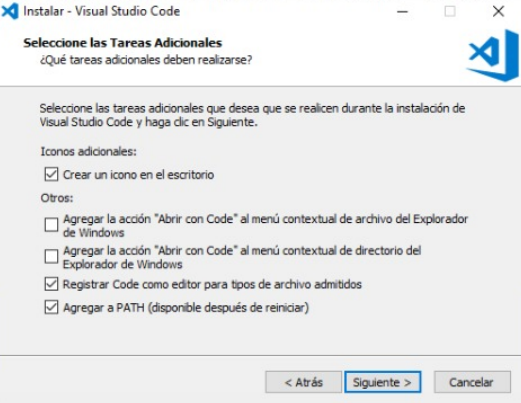
\includegraphics[width=1\textwidth]{./resources/3.png}
  \end{figure}
\end{frame}

\begin{frame}[fragile]{Instalación de editor de código}
  \textbf{VS Code en Windows}
  \begin{itemize}[<+(1)->]
    \item Click en siguiente hasta finalizar la instalación. Se ejecutará el programa.
  \end{itemize}
  \begin{figure}
    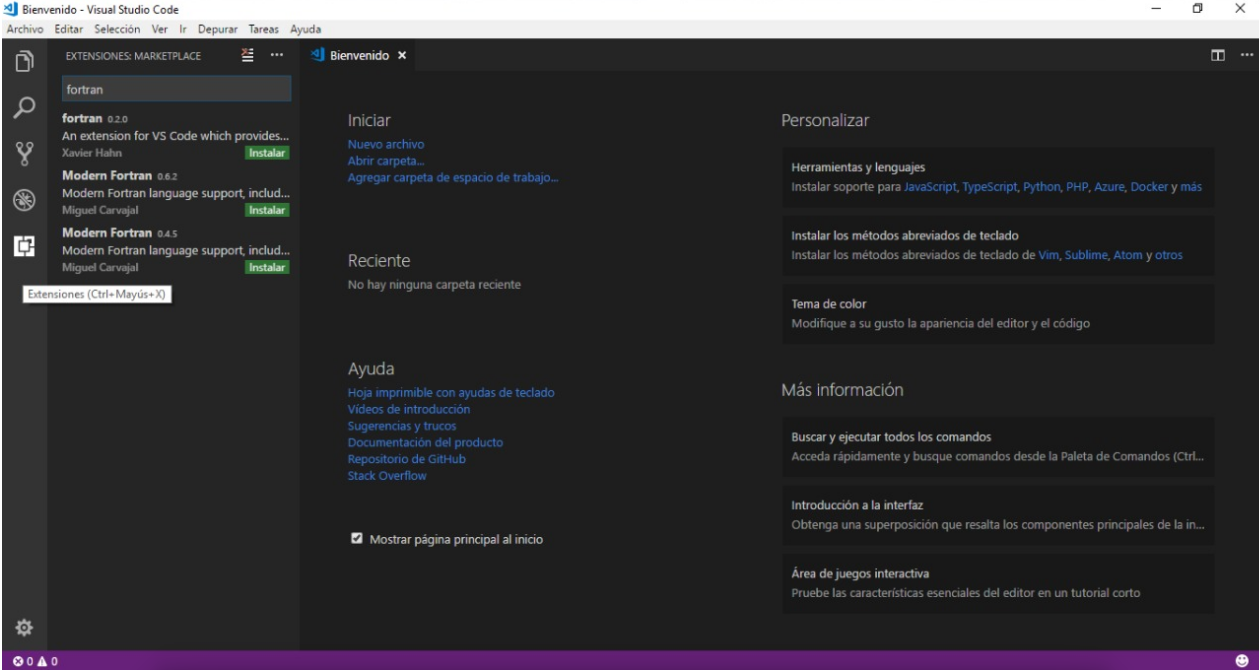
\includegraphics[width=1\textwidth]{./resources/4.png}
  \end{figure}
\end{frame}

\begin{frame}[fragile]{Instalación de compilador y debuger}
 \textbf{Instalación del compilador TDM-GCC}
 \begin{itemize}[<+(1)->]
  \item Descargar el paquete TDM-GCC según la versión de windows (32-64 bits) en \url{http://tdm-gcc.tdragon.net/}
  \item asdasd
 \end{itemize}
\end{frame}

